\documentclass{article}
% Change "article" to "report" to get rid of page number on title page
\usepackage{amsmath,amsfonts,amsthm,amssymb}
\usepackage{setspace}
\usepackage{Tabbing}
\usepackage{fancyhdr}
\usepackage{lastpage}
\usepackage{extramarks}
\usepackage{url}
\usepackage{chngpage}
\usepackage{longtable}
\usepackage{soul,color}
\usepackage{graphicx,float,wrapfig}
\usepackage{enumitem}
\usepackage{morefloats}
\usepackage{multirow}
\usepackage{multicol}
\usepackage{indentfirst}
\usepackage{lscape}
\usepackage{pdflscape}
\usepackage{natbib}
\usepackage{algorithm}
\usepackage{algorithmic}
\usepackage[toc,page]{appendix}
\providecommand{\e}[1]{\ensuremath{\times 10^{#1} \times}}

% In case you need to adjust margins:
\topmargin=-0.45in      % used for overleaf
%\topmargin=0.25in      % used for mac
\evensidemargin=0in     %
\oddsidemargin=0in      %
\textwidth=6.5in        %
%\textheight=9.75in       % used for mac
\textheight=9.25in       % used for overleaf
\headsep=0.25in         %

% Homework Specific Information
\newcommand{\hmwkTitle}{Progress Report 2}
\newcommand{\hmwkDueDate}{Monday,\ November\  5,\ 2018}
\newcommand{\hmwkClass}{Final Project}
\newcommand{\hmwkClassTime}{CSE 597}
\newcommand{\hmwkAuthorName}{Sahithi\ Rampalli}
\newcommand{\hmwkNames}{svr46}

% Setup the header and footer
\pagestyle{fancy}
\lhead{\hmwkNames}
\rhead{\hmwkClassTime: \hmwkTitle} 
\cfoot{Page\ \thepage\ of\ \pageref{LastPage}}
\renewcommand\headrulewidth{0.4pt}
\renewcommand\footrulewidth{0.4pt}

%%%%%%%%%%%%%%%%%%%%%%%%%%%%%%%%%%%%%%%%%%%%%%%%%%%%%%%%%%%%%
% Make title

\title{\vspace{2in}\textmd{\textbf{\hmwkClass:\ \hmwkTitle}} \\
\vspace{0.1in}\large{ \hmwkClassTime}\vspace{3in}}

\author{\textbf{\hmwkAuthorName} \\ \vspace{0.1in}
\hmwkDueDate }
\date{} % to take away today's date

%%%%%%%%%%%%%%%%%%%%%%%%%%%%%%%%%%s%%%%%%%%%%%%%%%%%%%%%%%%%%%

\begin{document}
\begin{spacing}{1.1}
\maketitle

\newpage
\section*{Abstract}

This report is an extension of the previous report. I chose to build an optimized iterative solver for the discrete Poisson Equation on Cartesian grid. In the previous report, I implemented a serial conjugate gradient (CG) iterative solver for the same. In this report, I tried to further optimize it by investigating the possible parallelizations in the iterative solver. I use OpenMP framework to accomplish the same. In the following sections, I discuss in detail about the problem I am trying to solve, the choice of parallelization method, the performance of different variants of parallel CG and their comparisons. The results of this project will be used for our research work where we implemented conjugate gradient solver for the same problem on FPGA architecture \cite{FPGACG}. The aim is to compare the performance of the solver on different architectures including CPU and FPGA. Discrete Poisson Equation is used in various applications such as in computational fluid dynamics, theory of markov chains. A fast and efficient implementation of CG will be useful in accelerating many applications in the scientific community. In our research problem, we are trying to investigate various optimization techniques to come up with an efficient implementation of the solver which can be used in many scientific applications. It is more a mathematical problem than physical problem and we do not target a specific application.
  

\section{Problem of Interest}

    Finite difference numerical method is used to discretize the 2-dimensional Poisson equation. On an m{x}n grid, it takes the form
\[(\nabla^2	u)_{ij} = \dfrac{1}{dx^2}(u_{i+1,j} + u_{i-1,j} + u_{i,j+1} + u_{i,j-1} - 4u_{i,j} ) \] 
	Discrete Poisson equation arises in various fields of study such as heat flow, electrostatics, gravity, computational fluid dynamics, theory of markov chains and many more. They occur frequently in scientific computing, for instance, when solving partial diferential equations, in inexact newton methods for solving optimization problems in machine learning applications etc. The size of the grids on which the equation is applied can go as large as 10s or 100s of 1000s. For such large matrix sizes, it is clearly essential to parallelize and optimize the solvers. Hence, an efficient implementation of CG which can be used in various physical applications is necessary. For our research, we have not chosen a specific physical problem, but would like to contribute possible optimization techniques for this iterative solver. However, for the convergence test, we use a tolerance to control the number of iterations. \\
	Convergence criteria: I have chosen the tolerance to be of the order of $10^{-4}$ as this will ensure good accuracy for most applications involving discrete poisson equation. 
	The solver breaks when the logarithm of dot product of the residual values is greater than logarithm of the tolerance.
\[ delta = dotProduct(residual\_values); \epsilon = 0.0001 \]
\[ log_{10}(\sqrt{|delta|}) >= log_{10}(\epsilon) \] 
\\
	Since the matrix sizes are really large, direct solvers are usually not preferred as $A^{-1}$ computation or back filling will be quite expensive. Iterative methods like  Jacobi, SOR, Conjugate Gradients are used to solve discrete Poisson Equation \cite{Berkley1996}. Iterative methods use the idea of nearest-neighbour computation to solve the equation. SOR and CG take about the same number of steps. However, the advantage of CG over SOR is that CG can be used for larger class of problems. Methods like FFT and Multigrid can be faster than the iterative methods as they forward the information to points on the grid which are farther than the nearest neighbours. FFTs and multigrid are more specialized to solve problems like Poisson, unlike direct solvers like LU decomposition which is used to solve almost any linear system (non-singular). \cite{FFTPoisson}
	\\
	We have a simple MATLAB implementation of Conjugate Gradient. We used it to compare the accuracy of our FPGA implementation. I have also used it to compare the accuracy of direct solver, serial and parallel CG implementations. A pseudo code of CG is shown in algorithm \ref{algoCG}
	
\begin{algorithm}[H]

%\begin{multicols}{2}
\begin{algorithmic}[1]
%\caption{function [A, x, b] = CG(A, b)}

%\label{alg:seq}
\STATE $n = \text{size}(A,1)$ 
\STATE $x = \text{zeros}(n,1)$
%\STATE $resVec = [\hspace{1mm}]$
\STATE $r_{\text{old}} = b$ ; $p = r_{\text{old}}$ ; $j = 1$
\FOR{$i=1$ until convergence}
\STATE $z = A*p$ 
\STATE ${\alpha} = (r_{\text{old}}, r_{\text{old}})/(z, p)$
\STATE $x = x + \alpha * p$ 
\STATE $r = r_{old} - \alpha * z$
\STATE $\beta = (r, r) \, / \, (r_{\text{old}}, r_{\text{old}})$
\STATE $p = r + \beta* p$;
\STATE $r_{\text{old}} = r$
%\STATE $resVec = [resVec, norm(A * x - b)]$ 
%\STATE $j \gets j + 1$	
\ENDFOR
%\STATE $its = j$
\end{algorithmic}
%\end{multicols}
\caption{\label{algoCG} function [A, x, b] = stdCG(A, b)} 
\end{algorithm}


\section{Parallelization}

    The performance of the serial iterative solvers was discussed in detail in the previous report. There is a lot of scope for parallelization in CG as many operations are point-wise operations like dot-product of vectors, vector addition and subtraction. I chose to use OpenMP framework for parallelizing the CG as it is quite intuitive in the first observation that the operations can be easily distributed among multiple threads and can be accumulated at the end. Also, as taught in class, OpenMP framework has simple directives which leverage the implementation aspects and aptly portray the architecture we wish to realize. The matrix multiplication operation in line 5 of \ref{algoCG} is realized as a stencil operation applied on vector $p$ instead of a matrix multiplication operation. The stencil will be:
\begin{tabular}{|c|c|c|}
\hline
0 & -1 & 0\\ \hline
-1 & 4 & -1 \\ \hline
0 & -1 & 0 \\ \hline
\end{tabular}

This can be very easily deduced from the discrete poisson form shown in section 1.  This stencil operation can also be parallelized using OpenMP.
    \\
    pthread Library: We can use the pthread library of C/C++ to accomplish the same. In fact, OpenMP directives can be directly mapped to the pthread functions. However, from programming point of you, OpenMP is simple and easy to use and keeps the code less complex.
    \\
    \\
    MPI: I propose a parallelization technique on stencil operation using MPI. Please note that the stencil operation is the first operation performed in every iteration of CG. We can scatter the vector, on which stencil is applied, among multiple cores using MPI\_SCATTER   and gather the final result after the operation using MPI\_GATHER. This can be applied to all other operations in CG. However, the OpenMP implementation is almost equivalent to this idea.  Hence, I have not evaluated/analyzed the CG implementation using MPI.
    \\
    \\
    MapReduce: In section 3.2, I discuss an alternative approach to parallelize CG. Though I have not used the MapReduce framework, I implemented an equivalent way to parallelize the stencil operation. In this approach, I divide the computation grid on which the stencil is applied, into 4 blocks (for 4 threads), perform stencil operation parallely on individual blocks and then accumulate the result into a shared grid. A similar idea is applicable for rest of the vector operations - dot product, vector addition and subtraction. Due to the simplicity and directness of OpenMP, I used that framework. 
    \\
    \\
    PGAS: As I have used C++ to implement the direct and iterative solvers for Project Report #1, I started with applying simple OpenMP directives to the existing code to identify which parts of the code can be parallelized. Later, I did not switch to a new language PGAS. PGAS is relavant to my implementation and partially shares the same idea as my implementation.
    
   
    The simple point-wise operations - dot product, vector addition and subtraction - can be applied on part of the vectors by individual threads. No thread communication is required for these point-wise operations. This can be achieved using simple directives in OpenMP. It is worth nothing that the result of the dot product operation has to accumulated in a single shared variable. This can be achieved by accumulating the result of each thread (applied on a part of the vector) in a private variable which can be added to the shared variable in a critical section. However, using the OpenMP directive, "reduction(+: shared variable)" also serves the purpose. 
 \\
        The stencil operation can also be parallelized. The threads can be scheduled statically on this operation. All threads apply stencil operations on different elements parallely. 
    
        All the major operations of each iteration are parallelized except for a few operations such as computing the alpha and beta in lines 6 and 9 of algorithm \ref{algoCG} respectively and computing the distance from tolerance after every iteration, which are critical sections of the code and need to be performed only by a single thread. 
        The percentage of parallel sections for different matrix dimensions is shown in table \ref{percent}.
\begin{table}[H]
\begin{center}
%\resizebox{\columnwidth}{!}{%
 \begin{tabular}{| c | c|} 
 \hline
Matrix dimension & Percentage of Parallel Code  \\ %[0.3ex] 
 \hline
1024 & 78.26 \\ %\hline
1600 &  73.6\\ %\hline 
10816 &  88.7\\ %[0.3ex]
 \hline
\end{tabular}%
%}
\end{center}
\caption{\label{percent} Percentage of Parallel Code.   } 
\end{table}

    
     There is no difference in the numerical setup for the iterative solver. The matrix $A$ is not stored, but every matrix operation is visualized as a stencil operation computed on a grid of dimension $n$ which is half of the matrix dimension ($N$). The vector $b$ is randomly generated. 
     The sample matrix sizes considered are $1024x1024$, $1600x1600$ and $10816x10816$. 
     The production matrix sizes are $250000x250000$ and $1000000x1000000$.
     For weak scaling, different set of sample matrix sizes were used as the ratio of number of cores to problem sizes have to remain constant. \\
     As mentioned in project report #1, the convergence of CG did not vary with change in the initialization of $x$. Hence, I considered the case where $x$ is initialized to zero. \\

\section{Profiling}

\subsection{Serial}
The tables  \ref{serial1024}, \ref{serial1600}, \ref{serial10816} show the profiles of the serial CG code for sample matrix dimensions 1024, 1600 and 10816 respectively. As expected, the Matmul (stencil operation) takes maximum percentage of time for any matrix dimension as the number of operations in this function are more than that in any other vector operation functions. 5 Operations are performed on each grid element as can be seen in the discrete Poisson equation in section 1. 

\begin{table}[H]
\begin{center}
%\resizebox{\columnwidth}{!}{%
 \begin{tabular}{| c | c|c|c|} 
 \hline
$Name$ & $Exclusive Time (msec)$ & $\% Time$ & $#Call$  \\ %[0.3ex] 
 \hline
Matmul & 0.788 & 12.2& 61\\ %\hline
VectorAdd1 &  0.296& 4.6 & 61\\ %\hline 
VectorAdd2 &  0.291& 4.5 & 61\\ %[0.3ex]
VectorSub &  0.295& 4.6 & 61\\ %[0.3ex]
DotProduct1 &  0.238& 3.7 & 61\\ %[0.3ex]
DotProduct2 &  0.239& 3.7& 61\\ %[0.3ex]
 \hline
\end{tabular}%
%}
\end{center}
\caption{\label{serial1024} Profile of Serial code for matrix size: 1024   } 
\end{table}

\begin{table}[H]
\begin{center}
%\resizebox{\columnwidth}{!}{%
 \begin{tabular}{| c | c|c|c|} 
 \hline
$Name$ & $Exclusive Time (msec)$ & $\% Time$ & $#Call$  \\ %[0.3ex] 
 \hline
Matmul & 1 & 17.9 & 82\\ %\hline
VectorAdd1 &  0.608 &6.7 & 82\\ %\hline 
VectorAdd2 &  0.596 & 6.5 & 82\\ %[0.3ex]
VectorSub &  0.606 & 6.6 & 82\\ %[0.3ex]
DotProduct1 &  0.487 & 5.3 & 82\\ %[0.3ex]
DotProduct2 &  0.488 & 5.3 & 82\\ %[0.3ex]
 \hline
\end{tabular}%
%}
\end{center}
\caption{\label{serial1600} Profile of Serial code for matrix size: 1600  } 
\end{table}

\begin{table}[H]
\begin{center}
%\resizebox{\columnwidth}{!}{%
 \begin{tabular}{| c | c|c|c|} 
 \hline
$Name$ & $Exclusive Time (msec)$ & $\% Time$ & $#Call$  \\ %[0.3ex] 
 \hline
Matmul & 26& 33.6 & 198\\ %\hline
VectorAdd1 &  9 &11.9 & 198\\ %\hline 
VectorAdd2 &  9 & 11.8 & 198\\ %[0.3ex]
VectorSub &  9& 12.1 & 198\\ %[0.3ex]
DotProduct1 &  7 & 9.5 & 198\\ %[0.3ex]
DotProduct2 &  7 & 9.5 & 198\\ %[0.3ex]
 \hline
\end{tabular}%
%}
\end{center}
\caption{\label{serial10816} Profile of Serial code for matrix size: 10816   } 
\end{table}


\\
Hence, I would like to focus on Matmul, the bottleneck, to improve performance. In order to perform the stencil operation, I currently use multiple conditional statements to check for boundary conditions while applying a stencil operation. An alternative way to perform stencil operation is to pad the given matrix with zeros on all sides and smoothly apply the stencil operation on the entire matrix. I implemented this alternative way and the profiles of the alternative serial CG code are shown in tables \ref{pad1024}, \ref{pad1600}, \ref{pad10816}. It can be seen that the Execution time of Matmul operation reduced for a given matrix size when padding is used. However, an extra function for padding has to be used. The aggregate time for execution of Matmul and Pad function is almost comparable to the previous Matmul function with conditional statements.

\begin{table}[H]
\begin{center}
%\resizebox{\columnwidth}{!}{%
 \begin{tabular}{| c | c|c|c|} 
 \hline
$Name$ & $Exclusive Time (msec)$ & $\% Time$ & $#Call$  \\ %[0.3ex] 
 \hline
Matmul & 0.506 & 8.3& 61\\ %\hline
PadFunction & 0.215 & 3.5& 61\\ %\hline

 \hline
\end{tabular}%
%}
\end{center}
\caption{\label{pad1024} Profile of Padded Serial code for matrix size: 1024   } 
\end{table}

\begin{table}[H]
\begin{center}
%\resizebox{\columnwidth}{!}{%
 \begin{tabular}{| c | c|c|c|} 
 \hline
$Name$ & $Exclusive Time (msec)$ & $\% Time$ & $#Call$  \\ %[0.3ex] 
 \hline
Matmul & 1 & 12.5 & 82\\ %\hline
PadFunction & 0.215 & 5.4& 82\\ %\hline
 \hline
\end{tabular}%
%}
\end{center}
\caption{\label{pad1600} Profile of Padded Serial code for matrix size: 1600  } 
\end{table}

\begin{table}[H]
\begin{center}
%\resizebox{\columnwidth}{!}{%
 \begin{tabular}{| c | c|c|c|} 
 \hline
$Name$ & $Exclusive Time (msec)$ & $\% Time$ & $#Call$  \\ %[0.3ex] 
 \hline
Matmul & 17& 22.7 & 198\\ %\hline
PadFunction & 7& 9.6 & 198\\ %\hline
 \hline
\end{tabular}%
%}
\end{center}
\caption{\label{pad10816} Profile of Padded Serial code for matrix size: 10816   } 
\end{table}

\\
I propose another technique to implement the stencil operation. The notion is to have some kind of pipeline design in Matmul. In this design, we use line buffers of size $3xGRID\_ COLUMN\_SIZE$ to cache every three rows of the grid. Note that, grid is the 2D vector representation on which the stencil is applied. The number three is chosen as the stencil dimension is three. Every element passes through the following pipeline stages.
\begin{itemize}
    \item The new element is updated in the line buffer.
    \item A current pointer is maintained to represent the locations on the line buffer where stencil is to be applied.
    \item The current pointer is used to update a window buffer of size $3x3$ (size of the stencil) which is the buffer on which stencil is applied.
    \item Finally, the stencil is applied on the window buffer.
\end{itemize}
We have used a similar pipelined approach in our FPGA implementation of CG. Please refer to the section III-B of \cite{FPGACG} for a better explanation. However, I have not included the evaluation of this method in the report.

\subsection{Parallel}

The profiles of parallel CG code for sample matrix sizes 1024, 1600 and 10816 using 4 threads are shown in tables \ref{ll1024}, \ref{ll1600}, \ref{ll10816} respectively. The Exclusive Time shown is mean of the exclusive time of each thread in a function. It can be seen that Matmul still takes the maximum amount of time among all functions. This is expected as the number of operations are split equally among all threads in any function. The total number of operations per thread has reduced. However, the number of operations in Matmul is still greater than that in other functions for a given thread. I have used static scheduling during parallelization as all threads perform similar operation. 

\begin{table}[H]
\begin{center}
%\resizebox{\columnwidth}{!}{%
 \begin{tabular}{| c | c|} 
 \hline
$Name$ & $Mean Exclusive Time (msec)$   \\ %[0.3ex] 
 \hline
Matmul & 0.26 \\ %\hline
VectorAdd1 &  0.148 \\ %\hline 
VectorAdd2 &  0.15\\ %[0.3ex]
VectorSub &  0.148\\ %[0.3ex]
DotProduct1 &  0.127\\ %[0.3ex]
DotProduct2 &  0.131\\ %[0.3ex]
 \hline
\end{tabular}%
%}
\end{center}
\caption{\label{ll1024} Mean Exclusive Time in msec of Parallel code for matrix size: 1024 using 4 threads. } 
\end{table}

\begin{table}[H]
\begin{center}
%\resizebox{\columnwidth}{!}{%
 \begin{tabular}{| c | c|} 
 \hline
$Name$ & $Mean Exclusive Time (msec)$   \\ %[0.3ex] 
 \hline
Matmul & 0.476 \\ %\hline
VectorAdd1 &  0.267 \\ %\hline 
VectorAdd2 &  0.278\\ %[0.3ex]
VectorSub &  0.258\\ %[0.3ex]
DotProduct1 &  0.224\\ %[0.3ex]
DotProduct2 &  0.22\\ %[0.3ex]
 \hline
\end{tabular}%
%}
\end{center}
\caption{\label{ll1600} Mean Exclusive Time in msec of Parallel code for matrix size: 1600 using 4 threads. } 
\end{table}

\begin{table}[H]
\begin{center}
%\resizebox{\columnwidth}{!}{%
 \begin{tabular}{| c | c|} 
 \hline
$Name$ & $Mean Exclusive Time (msec)$   \\ %[0.3ex] 
 \hline
Matmul & 6 \\ %\hline
VectorAdd1 &  3 \\ %\hline 
VectorAdd2 &  3\\ %[0.3ex]
VectorSub &  3\\ %[0.3ex]
DotProduct1 &  2\\ %[0.3ex]
DotProduct2 &  2\\ %[0.3ex]
 \hline
\end{tabular}%
%}
\end{center}
\caption{\label{ll10816} Mean Exclusive Time in msec of Parallel code for matrix size: 10816 using 4 threads. } 
\end{table}

The speedup of the parallel code over serial code for all sample matrix sizes is shown in table \ref{compspedup}. It can be noticed that parallel code is performing better than serial code for all sample matrix sizes. Also, the speedup is increasing with the increase in matrix dimensions. This is because for smaller matrix sizes, the communication overhead dominates the thread level parallelism which is compensated in case of larger matrices.
\begin{table}[H]
\begin{center}
%\resizebox{\columnwidth}{!}{%
 \begin{tabular}{| c | c|c|c|} 
 \hline
$Name$ & Speedup (N=1024) & Speedup (N=1600) & Speedup (N=10816)    \\ %[0.3ex] 
 \hline
Matmul & 3.03 &  2.1 & 4.33 \\ %\hline
VectorAdd1 &  2  &2.27   & 3 \\ %\hline 
VectorAdd2 &  1.94 &  2.14 &3 \\ %[0.3ex]
VectorSub &  1.99 &  2.35 & 3\\ %[0.3ex]
DotProduct1 &  1.87 &  2.17 &3.5 \\ %[0.3ex]
DotProduct2 &  1.82 &  2.22 & 3.5\\ %[0.3ex]
 \hline
\end{tabular}%
%}
\end{center}
\caption{\label{compspedup} Speedup of parallel code over serial code for sample matrix sizes.} 
\end{table}
\\
The table shows the time and memory estimates for production size matrix dimensions 250000 and 1000000, when run on 12 threads. The memory usage is obtained using the 'top' unix command.
\begin{table}[H]
\begin{center}
%\resizebox{\columnwidth}{!}{%
 \begin{tabular}{| c | c|c|} 
 \hline
 N & Exec Time (sec) & Memory (MB)   \\ %[0.3ex] 
 \hline
250000 & 0.8 & 29.3 \\ %\hline
1000000 & 6.6  & 69.3 \\ %\hline 

 \hline
\end{tabular}%
%}
\end{center}
\caption{\label{compspedup} Estimate of execution time and memory for production matrix dimensions when run on 12 threads.} 
\end{table}

As Matmul is taking maximum percentage of time. I tried to optimize this function. The stencil operation can also be parallelized by partitioning the computation grid such that the stencil operation is applied on each partition by individual threads (called Partitioned Parallel Code). I partitioned the grid into 4 blocks, each to be executed by a thread. Each block shares a row a neighbouring block and a column with a neighbouring block. The data of each partition is copied to a private data structure of each thread (called Copy Partial Data). The boundary data is copied to private buffers of each thread (called Copy Boundary Data).  Hence, the stencil operation is applied on individual blocks (called Partial Matmul). After the operation is performed, all threads write their outputs to a shared data structure (called Accumulate Output). The idea behind this modification is to investigate whether having private data structures for each thread will lead to better performance as the private data structures will be stored in the private caches of each cores. In the previous case, OpenMP directive was used to assign tasks to each thread to be performed on a shared memory. Though the number of stencil operations is same in both the cases, I wanted to investigate if manually partitioning the data will be more advantageous than having a shared data structure.  Table \ref{partition} shows the profile of the modified stencil operation. Though the partial Matmul operation performs better than the usual Matmul, the aggregate of Partial Matmul, pre-processing and post-processing is worse than Matmul for all matrix sizes.


\begin{table}[H]
\begin{center}
%\resizebox{\columnwidth}{!}{%
 \begin{tabular}{| c | c|c|c|} 
 \hline
$Name$ & Mean Time msec (1024) & Mean Time msec (1600) & Mean Time msec (10816)    \\ %[0.3ex]
 \hline
Partial Matmul & 0.147 &  0.297 & 4.26 \\ %\hline
Copy Partial Data & 0.117 &  0.188 & 2.43 \\ %\hline
Copy Boundary Data & 0.0253 & 0.036 & 0.146 \\ %\hline
Accumulate Output & 0.12 &  0.17 & 1.827 \\ %\hline
\cline{2-4}
Aggregate & 0.4093& 0.695 & 8.67\\%\hline
 \hline
\end{tabular}%
%}
\end{center}
\caption{\label{partition} Mean Time in msec of Partitioned Parallel code for matrix sizes 1024, 1600 and 10816. } 
\end{table}
\\
more suggestions

\section{Scaling}

\subsection{Strong Scaling}
In order to compute the strong scaling efficiency, I used 20 cores of Intel IvyBridge compute node, computed the the execution times of each problem size with varying number of cores from 1 to 20 (called \#Cores). Finally, efficiency of $x$ number of cores is computed as Speedup of $x$ number of cores over 1 core, averaged over $\#Cores$.
The plot of efficiency of parallel code for matrix sizes 1600 and 10816, for 20 cores, is shown in figure \ref{eff}. It can be seen that the efficiency decreases with the increase in number of cores. Single core has the maximum efficiency. Also, the efficiency is better for large matrix size as more percentage of resources are used in case of large matrix sizes. 


\begin{center}
	\begin{figure}[H]
	\centering
       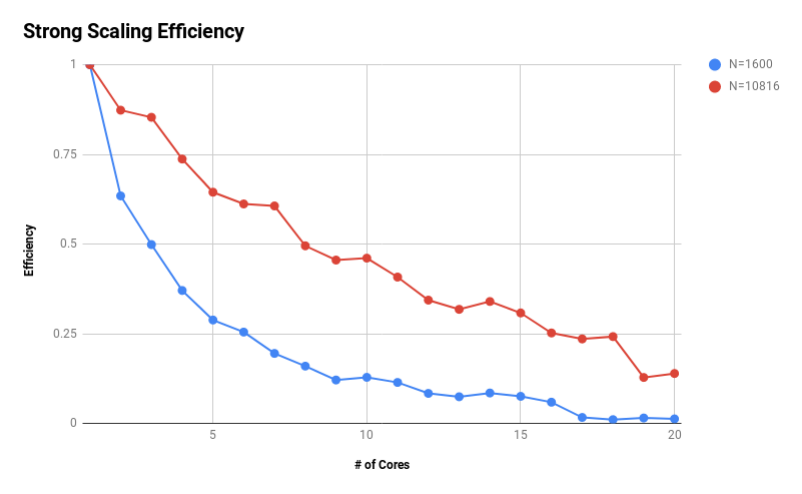
\includegraphics[scale=.40]{efficiency.png}
        \caption{\label{eff} Efficiency of parallel code for matrix sizes 1600 and 10816.} 
	\end{figure}
\end{center}

Figure \ref{Speedup} shows the speedup of parallel code for matrix sizes 1600 and 10816 for 20 cores. The speedup decreases rapidly beyond certain number of cores. This is because of communication overhead among cores and the thread handling (creation, joining etc) is higher for more number of cores and it dominates the parallelism. It can be seen that the speedup for larger matrix is more than that for smaller matrix. This is because the communication overhead is amortized over the matrix size. 

\begin{center}
	\begin{figure}[H]
	\centering
       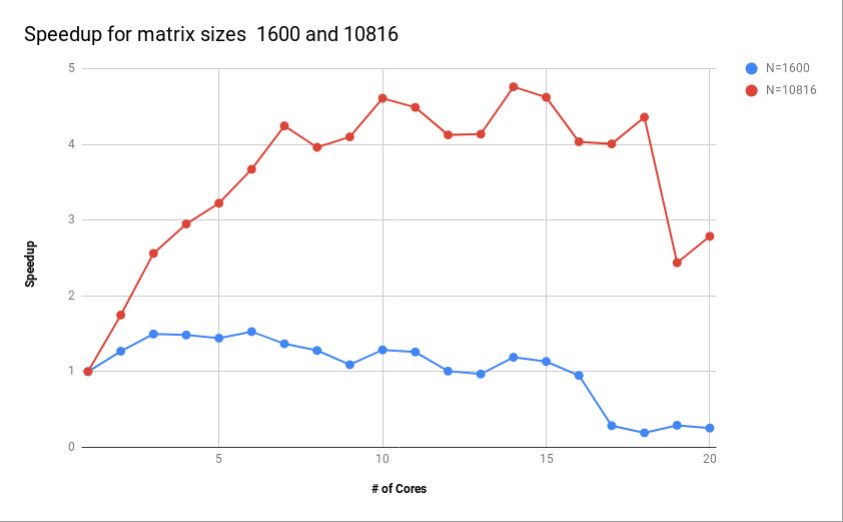
\includegraphics[scale=.40]{speedup.png}
        \caption{\label{Speedup} Speedup of parallel code for matrix sizes 1600 and 10816.} 
	\end{figure}
\end{center}


\begin{itemize}
    \item If speed is the concern, 6 and 14 cores would be best suitable for problems of size 1600 and 10816 respectively. 
    \item For perfectly efficient use of resources, single core would give the best results for any matrix size.
    \item For our research purposes, I would choose a reasonably efficient problem with close to maximum speedup. Speedup is more important for my case. Thus, 3 cores would be appropriate for matrix size 1600 and 10 cores would be appropriate for matrix size 10816. The efficiency for both are close to 0.5.
\end{itemize}
Thus, the optimal starting point for problem sizes greater than or equal to 10816 would be 10 cores. \\
\\
The plots \ref{Speedup1600} and \ref{Speedup10816} show the speedup of parallel code for matrix sizes 1600 and 10816 along with the theoretical speedup given by Amdahl's law and the ideal speedup which is equal to the number of cores used. The percentage of parallel code for matrix sizes 1600 and 10816 are 73.6\%  and 88.7\% respectively. As the matrix size increases, the speedup is closer to the theoretical speedup from Amdahl's law for more number of cores. In case of matrix size 1600, the obtained speedup is close to the theoretical speedup upto 2 cores. In case of matrix size 10816, the obtained speedup is close to the theoretical speedup upto 10 cores. \\
In the plot of speedup for matrix 10816, the curve has multiple local minima. A decrease in speedup beyond certain number of cores is expected as the communication overhead could be more dominant than the parallelism effect. However, we can find some local minima even for smaller number of cores. For instance, the speedup for 8 and 9 cores is less than that for 10 cores. The reason could probably be that the matrix dimension is not an exact multiple of number of cores and the code uses static scheduling. Hence, all cores may not finish at the same time and some cores have to wait for the rest of the cores to finish wherever there is a barrier.

\begin{center}
	\begin{figure}[H]
	\centering
       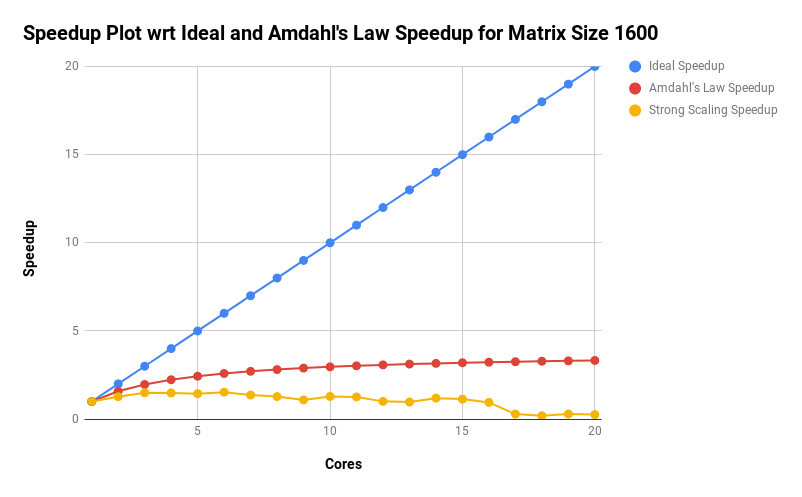
\includegraphics[scale=.40]{speedup1600.png}
        \caption{\label{Speedup1600} Speedup of parallel code for matrix size 1600 along with theoretical speedup given by Amdahl's law and the ideal speedup.} 
	\end{figure}
\end{center}

\begin{center}
	\begin{figure}[H]
	\centering
       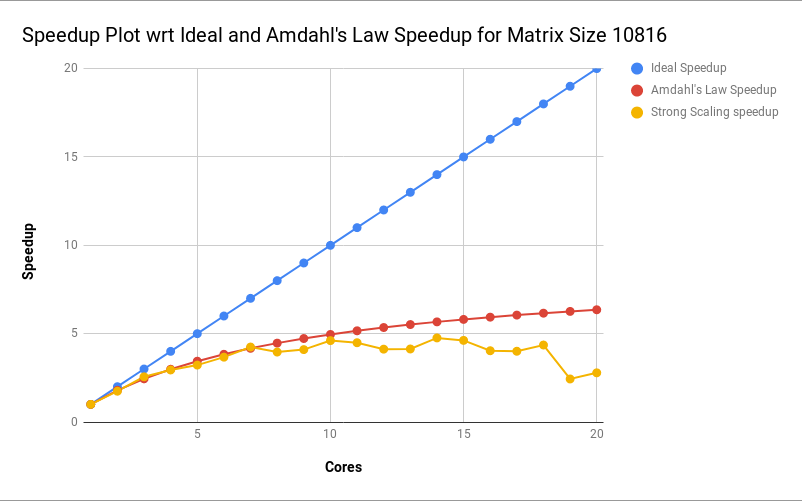
\includegraphics[scale=.40]{speedup10816.png}
        \caption{\label{Speedup10816} Speedup of parallel code for matrix size 160816 along with theoretical speedup given by Amdahl's law and the ideal speedup..} 
	\end{figure}
\end{center}


\subsection{Weak Scaling}
The weak scaling efficiency is computed as speedup of $x$ number of cores over 1 core. 
The Weak scaling efficiency plot is shown in figure \ref{weakscaling}. The horizontal axis represents the tuple (cores, matrix size). The matrix sizes here are different as the ratio of cores and matrix size has to remain constant in the plot. Clearly, the efficiency decreases with the increase in number of cores used and hence, the matrix size.


\begin{center}
	\begin{figure}[H]
	\centering
       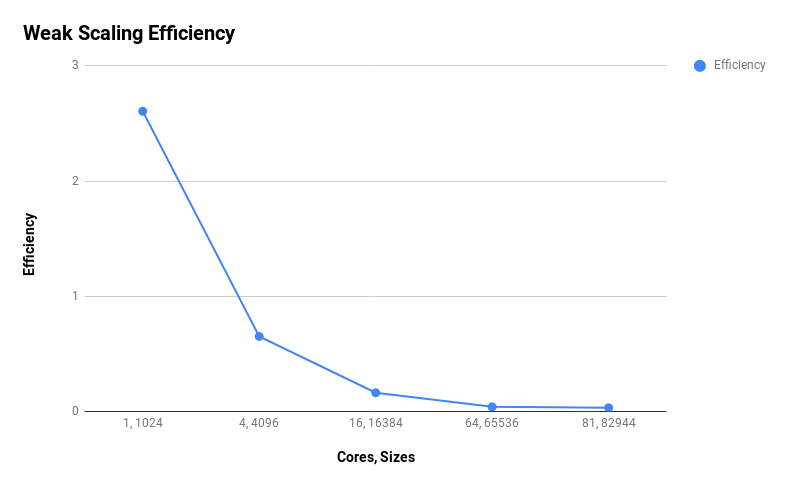
\includegraphics[scale=.40]{weakscaling.png}
        \caption{\label{weakscaling} Weak Scaling Efficiency plot .} 
	\end{figure}
\end{center}


\section{Discussion and Conclusions}

In this report, I have explained the need for an efficient implementation of Conjugate Gradient iterative solver for Discrete Poisson problem, investigated some possible methods to improve the performance of serial code. Later, I came up with possible parallelization techniques that could be applied for vector operations and stencil operation and discussed about further possible parallelism in the code. We have then observed the speedup of parallel code over the serial code for 4 thread-parallelism. We have seen the strong scaling efficiency and speedup of the parallel code over 20 cores and compared the speedup with the theoretical speedup and ideal speedup. 

\\
I used OpenMP framework for parallelization. As discussed in section-2, OpenMP pragmas make it simple to apply and appropriately realize the parallelism in the CG implementation. Also, the reduction pragma can be directly applied for dot product operation and the grid decompositions can directly given as tasks to individual threads. \\
\\
In conclusion, with an efficiency of about 50\%, the optimal number of cores would be 10 for matrix size of 10816 and around 10-14 for production matrix dimensions. 
\\
For the final report, I would like to incorporate the other possible parallelizations in the code and compare the various approaches. If possible, I would like to use other frameworks like MPI and MapReduce and compare the performances of each of the codes. 


\newpage
\begin{appendices}

\section{Acknowledgements}

I would like to acknowledge my advisor Dr. Pawan Kumar, IIIT-Hyderabad, India for guiding me to work on conjugate gradient solver for discrete poisson equation on different architectures. I would like to acknowledge my class mates, Chirag Satish and Amatur Rahman, for helping me fix some implementation errors and clarifying some doubts regarding strong and weak scaling.

\section{Code}

The code is publicly accessible on GitHub. URL: https://github.com/sahithi-rv/ProjectReport2.
One can do git clone https://github.com/sahithi-rv/ProjectReport2.git to obtain the code repository.
\subsection{File names and Descriptions}
\begin{itemize}
\item Serial Codes directory - iter\_serial.
\begin{itemize}
    \item cg.cpp - Pure CG serial code.
    \item cg\_pad.cpp - Modified CG code with padding described in section 3.1
\end{itemize}
\item Parallel Codes directory - iter\_parallel.
\begin{itemize}
    \item cg\_omp3.cpp - Main Parallel CG code.
    \item cg\_omp\_next.cpp - modified CG with partial Matmul as discussed in section 3.2
    \item cg\_omp\_tau.cpp - Added tau profiler clauses to obtain profiles of Parallel code.
\end{itemize}
\item Test Matrices directory - test\_matrices
\begin{itemize}
    \item The file names have matrix sizes to indicate the file that needs to be passed as argument for a required matrix size.
\end{itemize}
\item parallel\_profile\_output.txt - profile of parallel code for 4 threads
\item serial\_profile\_output.txt - profile of serial code
\item profile\_serial\_pad\_output.txt - profile of modified padded serial code.

\end{itemize}

\subsection{Compile and Run Instructions}
\begin{itemize}
    \item To compile and serial code to obtain profile
    \begin{itemize}
        \item cd iter\_serial
        \item module load gcc/5.3.1
        \item module load tau/2.27
        \item tau\_cxx.sh -std=c++11 -g -o tauperf\_serial ./cg.cpp
        \item tau\_exec ./tauperf\_serial  ../test\_matrices/b1024 32
        \item tau\_exec ./tauperf\_serial  ../test\_matrices/b1600 40
        \item tau\_exec ./tauperf\_serial  ../test\_matrices/b10816 104
        \item pprof
        \item The arguments are Test Matrix file and the square root of matrix dimensions.
    \end{itemize}
    \item In order to simply compile the code run `make cg` and execute as ./cg test\_file\_name and square root of matrix dimension. Note that the code should be compiled with -std=c++11 flag.
    \item Similar instructions should be run for modified padded serial code - cg\_pad.cpp
    \item To compile and run parallel code and obtain the profiles
    \begin{itemize}
        \item module purge
        \item rm profile*
        \item cd iter\_parallel
        \item module load gcc/5.3.1
        \item module use /storage/work/a/awl5173/toShare/tauOMP/tau
        \item module load adamsTauOMP\_2.27
        \item tau\_cxx.sh -std=c++11 -fopenmp -g -o cg\_omp\_tau cg\_omp\_tau.cpp
        \item ./cg\_omp\_tau ../test\_matrices/b1024 32 4
        \item ./cg\_omp\_tau ../test\_matrices/b1600 40 4
        \item ./cg\_omp\_tau ../test\_matrices/b10816 104 4
        \item pprof
        \item The results in section 3 are shown for 4 thread-parallelism.  The arguments are the test matrix file, square root of matrix dimensions and the number of threads.
    \end{itemize}
    \item Similar instructions should be run for modified parallel code - cg\_omp\_next.cpp
    \item In order to compile the code, run `make cg\_omp3` and execute as `./cg\_omp3 test\_file\_name, square root of matrix dimension and number of threads`.
    
\end{itemize}

The compute node used was the node with Intel Ivybridge processor (comp-sc-0063). For strong scaling, I used 20 cores and for weak scaling, I used 5 nodes each with 20 cores.


\section{Poster Draft - separate document}
The poster is attached along with the report.


\end{appendices}


\bibliographystyle{acm}
\bibliography{progressReport}

\end{spacing}

\end{document}

%%%%%%%%%%%%%%%%%%%%%%%%%%%%%%%%%%%%%%%%%%%%%%%%%%%%%%%%%%%%%}}
